\section{System State Notations} 
\label{sec:notations}
A sensible notation of a system aids implementation and consistent discussion of motion control systems. Vessel automation is a topic where robotic and maritime science overlap. System description of vessel systems from a control perspective is described in \citet{fossen2011handbook}, which are used as a foundation of the multi-vessel state description

\subsection{Single vessel state description}
For control purposes, ships are generally considered rigid bodies. A rigid body has 6 degrees of freedom (DOF) in which can all be evaluated or simplified to a reduced set of motions such as 3-DOF planar motion. For ships, this is commonly expressed according to the notation of \citet{sname1950nomenclature} with respect to various coordinate systems. Components of orientation, velocities and forces are shown in table \ref{tableSname}.

\begin{table}[h!]
	\centering
	\begin{tabular}{|l|l|l|l|l|}
		\hline
		DOF & & \begin{tabular}[c]{@{}l@{}}Positions and \\ Euler Angles\end{tabular} & \begin{tabular}[c]{@{}l@{}}Linear and \\ angular Velocities\end{tabular}   & \begin{tabular}[c]{@{}l@{}}Forces and \\ Moments\end{tabular}  \\ \hline
		1&	Surge      & x                    & u          & X                  \\ \hline
		2&	Sway       & y                    & v          & Y                  \\ \hline
		3&	Heave      & z                    & w          & Z                  \\ \hline
		4&	Roll       & $\phi $                 & p          & K                  \\ \hline
		5&	Pitch      & $\theta  $              & q          & M                  \\ \hline
		6&	Yaw        & $\psi  $                & r          & N                \\ \hline
		
	\end{tabular}
	\caption{SNAME notation for marine vessels}
	\label{tableSname}
\end{table}

A North-East-Down coordinate system will be used as reference to a global coordinate system as $\{n\}$, while a body fixed coordinate system is referred to with $\{b\}$. This body fixed frame defines the motion of the vessel, such that every position or speed of a vessel is defined in the motion of the body frame. Figure \ref{figsname} shows vessel motions expressed on the body fixed frame. Motion of surface vessels is commonly simplified to 3 degrees of freedom in the surface plane, as is shown in figure \ref{fig:delfiaBodyFrame1}. This assumes effects of heave, roll and pitch can be neglected. This simplification of planar motion is adopted for the developed control system in this paper as described in Chap. \ref{chap:sysDevelopent}. 

\begin{figure}[h!]
	\centering
	\makebox[\textwidth][c]{
		\begin{minipage}{0.45\textwidth}
	\centering
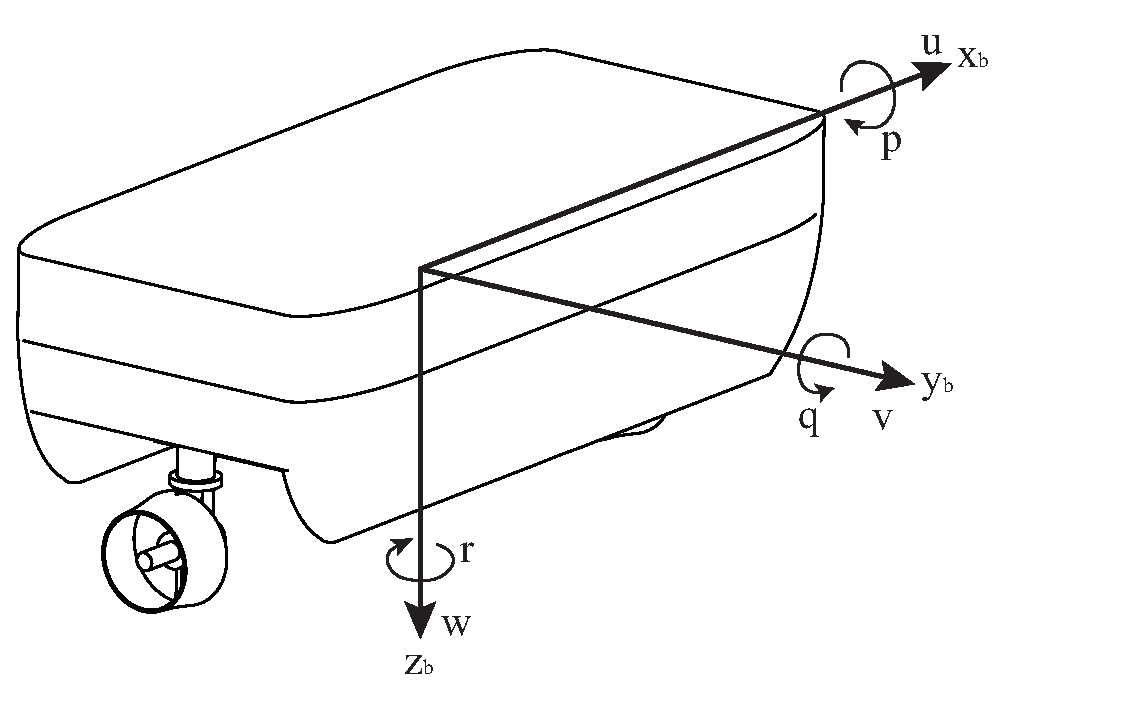
\includegraphics[width=1.0\textwidth]{DelfiaSname.eps}
\caption{Six degrees of motion depicted of a Delfia vessel expressed with respect to the body-fixed coordinate system $\{b\}$ in convention with \citet{sname1950nomenclature}}
\label{figsname}
		\end{minipage}\hfill
		\begin{minipage}{0.45\textwidth}
	\centering
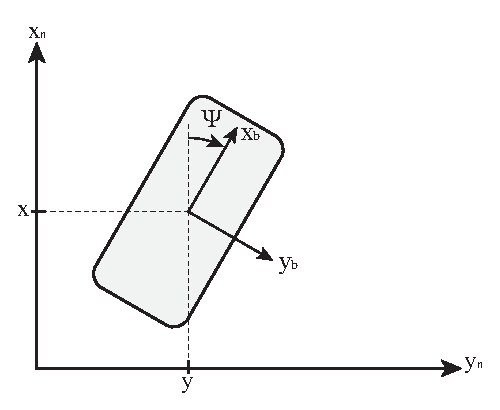
\includegraphics[width=1.0\textwidth]{delfia_bodyframe1.eps}
\caption{Three degrees of freedom depicted as only motion in the surface plane is considered}
\label{fig:delfiaBodyFrame1}
		\end{minipage}
	}
\end{figure}

Position, orientation, velocities, forces and moments are further noted as:
\begin{table}[H]
\centering
\begin{tabular}{lll}
		$\textbf{p}^{i}_{j} $ 			& = &  	Position of point $j$ expressed in coordinate system $\{i\}$ \\[5pt]
		$\Theta_{ij}$ 					& = & 	Euler angles between coordinate systems $\{i\}$ and $\{j\}$ \\[5pt]
		$ \textbf{v}^{k}_{i/j}$   		& = & 	Linear velocity of point i with respect to j expressed in coordinate system $\{k\}$ \\[5pt]
		$ \omega^{k}_{i/j}$   			& = &	Angular velocity of object i with respect to j expressed in coordinate system $\{k\}$  \\[5pt]
		$\boldmath{f}^{i}_{j} $ 	   	& = &	Force with line of action through point $j$ expressed in coordinate system $\{i\}$ \\[5pt]
		$\boldmath{m}^{i}_{j} $   		& = & 	Moment about point $j$ expressed in coordinate system $\{i\}$
\end{tabular}
\end{table}

As a result of the reduction from 6 to 3 degrees of freedom, vectorial expressions of our system become:
\begin{table}[H]
	\centering
	\begin{tabular}{llllllll}
		NED position & $\textbf{p}^{n}_{b} $ & = & $  \begin{bmatrix} x^{n}_{b} \\[5pt] y^{n}_{b} \end{bmatrix}$ & 
		Attitude (Euler angles) & $\Theta_{nb} $ & = & $ \begin{bmatrix} \Psi^n_b \end{bmatrix}$   \\[20pt] %\begin{bmatrix} N \\ E \end{bmatrix} =
		\begin{tabular}[c]{@{}l@{}}Body-fixed \\ linear velocity \end{tabular} & $ \textbf{v}^{b}_{b/n} $ & = & $ \begin{bmatrix} u \\ v \end{bmatrix} $ & 
		\begin{tabular}[c]{@{}l@{}}Body-fixed \\ angular velocity \end{tabular} & $ \omega^{b}_{b/n} $ & = & $ \begin{bmatrix} r \end{bmatrix} $ \\[20pt]
		\begin{tabular}[c]{@{}l@{}}Body-fixed \\ force \end{tabular} & $\boldmath{f}^{b}_{b} $ & = & $ \begin{bmatrix} X \\ Y \end{bmatrix} $ & 
		\begin{tabular}[c]{@{}l@{}}Body-fixed \\ moment \end{tabular} & $\boldmath{m}^{b}_{b} $ & = & $ \begin{bmatrix} N \end{bmatrix} $ 
	\end{tabular}
\end{table}


General motion of vessels in 3 degrees of freedom are described by the following generalized positions and velocities \cite{fossen2011handbook}

\begin{equation}
	\eta = \begin{bmatrix} \textbf{p}^{n}_{b} \\[8pt]  \Theta_{nb} \end{bmatrix} = \begin{bmatrix} x^{n}_{b} \\[8pt]  y^{n}_{b} \\[8pt] \Psi^n_b \end{bmatrix}
	\label{generalizedPos1}
\end{equation}

\begin{equation}
	\nu = \begin{bmatrix} \textbf{v}^{b}_{b/n} \\[8pt]  \omega^{b}_{b/n} \end{bmatrix} = \begin{bmatrix} u\\v\\r \end{bmatrix}
	\label{generalizedVel1}
\end{equation}

\begin{equation}
	\tau = \begin{bmatrix} \boldmath{f}^{b}_{b} \\[8pt]  \boldmath{m}^{b}_{b} \end{bmatrix} = \begin{bmatrix} X \\ Y \\ N \end{bmatrix}
	\label{generalizedFor1}
\end{equation}

Where $\eta$ describes orientation, $\nu$ describes velocities and $\tau$ describes forces acting upon the system. 
To avoid clutter, when it is deemed clear to in which reference frame a position or velocity is expressed, the subscript and superscript will not always be shown. This is for instance the case for generalized positions as in equation \ref{generalizedPos1} that is most of the time with respect to $\{n\}$ such that it is just expressed in $ [x,y,\Psi]^\top$. By default, $ \nu$, $\tau$ are expressed in $\{b\}$, and $\eta$ is described in $\{n\}$.

Velocities expressed in $\{b\}$ and $\{n\}$ frame are related as:

\begin{equation}
\dot{\eta} = R(\Psi)\nu
\end{equation}

Where $R$ is the rotation matrix of $\Psi$ around the z axis. For pure motion in the 3 surface plane degrees of freedom, this becomes:

\begin{equation}
R(\Psi) = \begin{bmatrix} cos(\Psi) & -sin(\Psi) & 0  \\ sin(\Psi) & cos(\Psi) & 0 \\ 0 & 0 & 1 \end{bmatrix}
\end{equation}

Coordinate system origin and centre of mass are referred to as:

\begin{table}[H]
	\centering
	\begin{tabular}{lll}
		$\textbf{o}_{i}^{j} $ 			& = &  	Origin of coordinate system $i$ expressed in coordinate system $\{j\}$ \\[10pt]
		$\textbf{p}_{cm}^{i} $ 			& = &  	Position of the centre of mass expressed in coordinate system $\{i\}$ \\
	\end{tabular}
\end{table}


\subsection{Multivessel system notation}
As fleet systems transition from describing a single vessel to a system of many, it becomes necessary to differentiate between local frames of different vessels. We change subscripts referencing to a single vessel to a notation for $n$ vessels. For example, referencing to a single body coordinate system as $\{b\}$ changes to $\{b1\},\{b2\},\{b2\} \dots \{bn\}$ in order to indicate which body frame is referenced to. Relative orientations and velocities are considered to become more relevant as vessels have to operate in proximity or even contact to realize assembly into platforms. Figure \ref{fig:localframeShowing} illustrates how position of a vessel can be described in a local body fixed frame, which may be more relevant and intuitive for automated assembly purposes. The position of origin of body 2 expressed in $\{b1\}$ illustrated in figure \ref{fig:localframeShowing} becomes:

\begin{equation}
\textbf{o}_{b1}^{b2} = \begin{bmatrix}x_{b1}^{b2} \\[10pt] y_{b1}^{b2} \end{bmatrix}
\end{equation}

Furthermore, the notations of motion shown in equation \ref{generalizedPos1}, \ref{generalizedVel1} and \ref{generalizedFor1} by default refer to a specific frame. Pose $\eta$ is expressed globally in $\{n\}$. Velocities $\nu$ and  forces $\tau$ are expressed in the body fixed frame $\{b\}$. It can be convenient to express motions to different frames as well. Take the example of two moving vessels docking to eachother while moving. To answer the question "How close is a vessel to a docking position?" a relative expression of position is required. The convention of subscripting to refer to a coordinate system is extended to $\eta$, $\nu$ and $\tau$ as well as follows:

\begin{equation}
\eta_b^n = \begin{bmatrix} \textbf{p}^{n}_{b} \\[8pt]  \Theta_{nb} \end{bmatrix} = \begin{bmatrix} x^{n}_{b} \\[8pt]  y^{n}_{b} \\[8pt] \Psi^n_b \end{bmatrix}
\label{generalizedPos2}
\end{equation}

Where the sub- and superscript of $\eta_b^n$ refer to object $b$ expressed in $\{n\}$. This convention allows expression of relative motion between vessels by writing $\eta_{b2}^{b1}$ which indicates pose of body 2 expressed in the local frame of body 1, also illustrated in \ref{fig:localframeShowing}. Note that velocities and forces are regularly referred to as "body-fixed", but that is not necessarily the case anymore with this convention. 

\begin{figure}[h!]
	\centering
	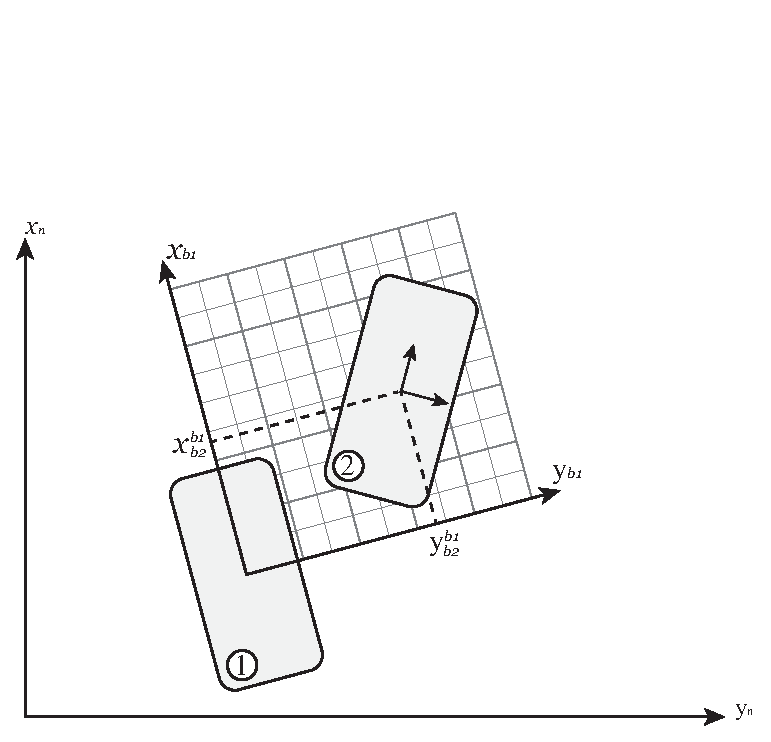
\includegraphics[width=0.6\textwidth]{localframeShowing.eps}
	\caption{Two vessels are shown from above, illustrating interpretation of expressing a module's state (of module 2) in another module's body-fixed coordinate system (of module 1).}
	\label{fig:localframeShowing}
\end{figure}
\newpage